%% LaTeX-Beamer template for KIT design
%% by Erik Burger, Christian Hammer
%% title picture by Klaus Krogmann
%%
%% version 2.1
%%
%% mostly compatible to KIT corporate design v2.0
%% http://intranet.kit.edu/gestaltungsrichtlinien.php
%%
%% Problems, bugs and comments to
%% burger@kit.edu

\documentclass[18pt]{beamer}

%% SLIDE FORMAT

% use 'beamerthemekit' for standard 4:3 ratio
% for widescreen slides (16:9), use 'beamerthemekitwide'

\usepackage{templates/beamerthemekit}
% \usepackage{templates/beamerthemekitwide}
\usepackage{graphicx}
%% TITLE PICTURE

% if a custom picture is to be used on the title page, copy it into the 'logos'
% directory, in the line below, replace 'mypicture' with the 
% filename (without extension) and uncomment the following line
% (picture proportions: 63 : 20 for standard, 169 : 40 for wide
% *.eps format if you use latex+dvips+ps2pdf, 
% *.jpg/*.png/*.pdf if you use pdflatex)

%\titleimage{mypicture}

%% TITLE LOGO

% for a custom logo on the front page, copy your file into the 'logos'
% directory, insert the filename in the line below and uncomment it

%\titlelogo{mylogo}

% (*.eps format if you use latex+dvips+ps2pdf,
% *.jpg/*.png/*.pdf if you use pdflatex)

%% TikZ INTEGRATION

% use these packages for PCM symbols and UML classes
% \usepackage{templates/tikzkit}
% \usepackage{templates/tikzuml}

% the presentation starts here

\title[Short title]{ICPC}
\subtitle{Graphen 3}
\author{Tobias, Julian, Jakob, Tobias}

\institute{ITI Wagner, IPD Tichy}

% Bibliography

\usepackage[citestyle=authoryear,bibstyle=numeric,hyperref,backend=biber]{biblatex}
\addbibresource{templates/example.bib}
\bibhang1em

\begin{document}

% change the following line to "ngerman" for German style date and logos
\selectlanguage{english}

%title page
\begin{frame}
\titlepage
\end{frame}

%table of contents
\begin{frame}{Outline/Gliederung}
\tableofcontents
\end{frame}

\section{Tobias}
\begin{frame}{Definiton Netzwerk}
\begin{itemize}
\item Quell- und  Senk- Knoten
\item Knoten haben Kapazit\"at
\end{itemize}
\end{frame}

\begin{frame}{Fluesse}
	\begin{itemize}
	\item fkt F:E-$>$R weist jeder Kante einen Flusswert zu
	\item Kapazit\"atskonfirmation
	\item Flusserhalt
	\item Wert eines Flusses
	\item Exzes
	\item je definiton, kurze erkl\"areung ggf. an einem Bild
	\end{itemize}
\end{frame}

\begin{frame}{Probleme zu Fl\"ussen}
	\begin{itemize}
		\item Schwierigeit im Erkennen der Aufgaben
		\item tauchen seit 2013 wieder auf, zählen zu "decider" Problemen
		\item eine beilspielaufgabe vorstellen, erkl\"aren warum das eine Flussaufgabe ist
	\end{itemize}
\end{frame}

\section{Jakob}
\begin{frame}{Augmentierender/erweiternder Weg}
	\begin{itemize}
		\item Erkl\"arung augmentierender/erweiternder Weg
	\end{itemize}
\end{frame}

\begin{frame}{Ford-Fulkerson + Bsp}
	\begin{itemize}
		\item Erklaerung Ford-Fulkerson
	\end{itemize}
	\begin{figure}
		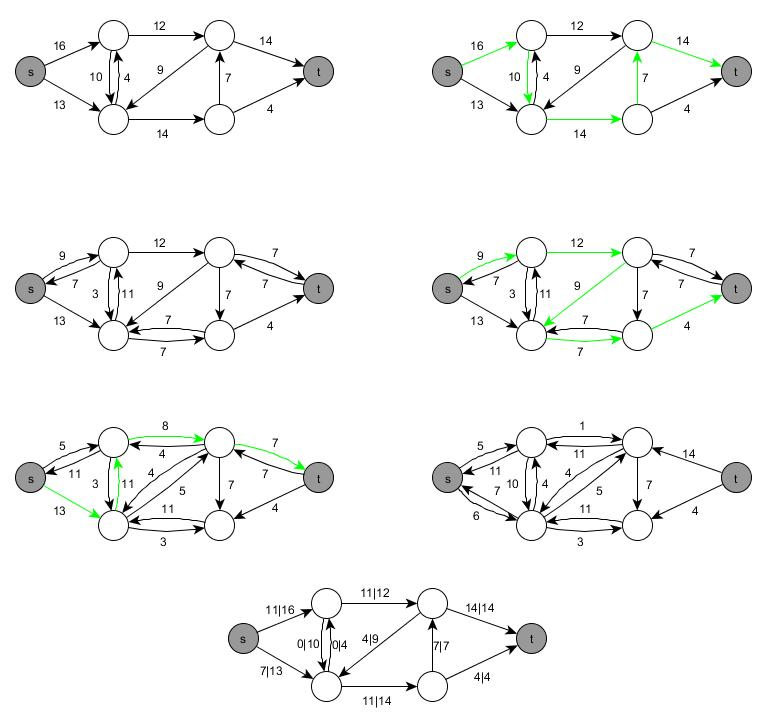
\includegraphics[width = 0.5\textwidth]{img/Jakob_Ford.jpg}
	\end{figure}
\end{frame}


\begin{frame}{Ford-Fulkerson - Warum schlecht}
	\begin{itemize}
		\item Laufzeit - nicht benutzen
	\end{itemize}
	\begin{figure}
		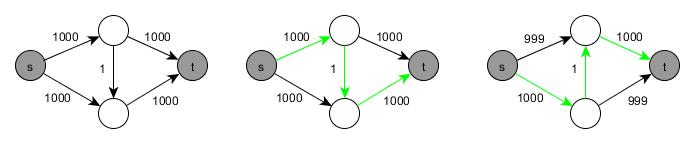
\includegraphics[width = 0.7\textwidth]{img/Jakob_Ford2.jpg}
	\end{figure}
\end{frame}


\begin{frame}{Edomnd-Karp Algorithmus}
	\begin{itemize}
		\item Pseudocode + Beispiel
	\end{itemize}
	\begin{figure}
		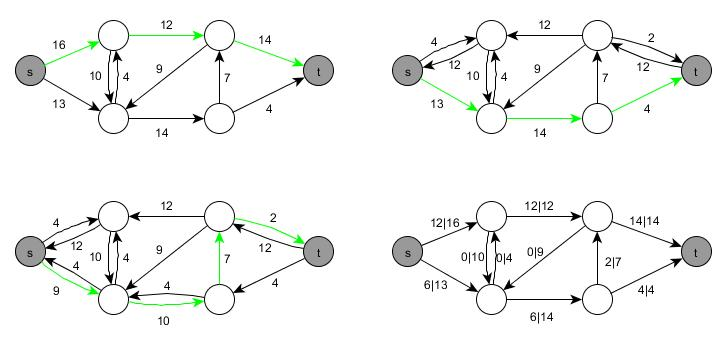
\includegraphics[width = \textwidth]{img/Jakob_Edmond.jpg}
	\end{figure}
	
	\begin{itemize}
		\item Implementierungsdetails
	\end{itemize}
\end{frame}


\section{Julian}
\begin{frame}{Max Flow/Min Cut theorem}
	\begin{itemize}
		\item Definiton der Schnittmenge C
		\item \"Uberlegungen, dass Max Flow = Min Cut
		\item Beispielanhand von S. 163 in Competitive Programming 3
	\end{itemize}
	\begin{figure}
		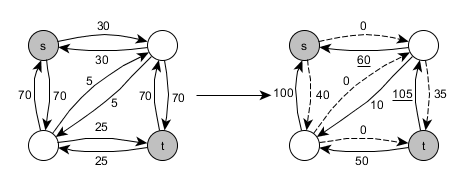
\includegraphics[width = \textwidth]{img/Julian_MaxMin.jpg}
	\end{figure}
\end{frame}

\begin{frame}{Multi-Quelle/Multi-Abfluss}
	\begin{itemize}
		\item Erl\"auterung der L\"osung anhand von Beispielen
	\end{itemize}
	\begin{figure}
		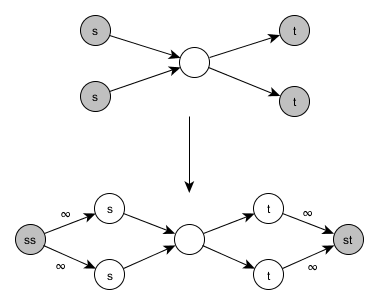
\includegraphics[width = 0.5\textwidth]{img/Julian_Multi.jpg}
	\end{figure}
\end{frame}


\begin{frame}{Knotenkapazit\"at}
	\begin{itemize}
		\item Aufl\"osen anhand von Bsp.
	\end{itemize}
	\begin{figure}
		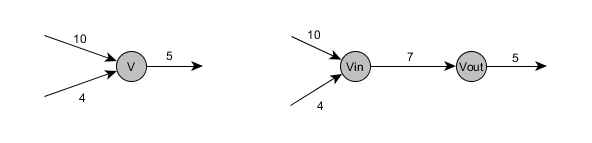
\includegraphics[width = 0.8\textwidth] {img/Julian_Kapazitaet.jpg}
	\end{figure}
\end{frame}


\begin{frame}{Modelierung}
	\begin{itemize}
		\item Probleme der Erkennung eines Max Flow Problems
		\item Herleiten einer beispielhaften l\"osung einer Modellierung anhand von UVa 11380
	\end{itemize}
\end{frame}


\section{Tobias T}
\begin{frame}{Bipartiter Graph}
	\begin{itemize}
		\item Bipartiter Graph
	\end{itemize}
	\begin{figure}
		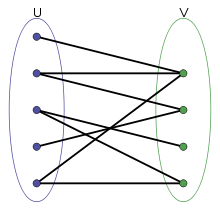
\includegraphics[width = 0.5\textwidth] {img/TobiasT_Bipartit.jpg}
	\end{figure}
\end{frame}

\begin{frame}{Matching}
	\begin{itemize}
		\item Definitionen: Matching, maximales Matching, kardinalit\"atsmaximales Matching, perfektes Matching
	\end{itemize}
	\begin{figure}
		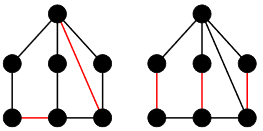
\includegraphics[width = 0.5\textwidth]{img/TobiasT_Matching.jpg}
	\end{figure}
\end{frame}


\begin{frame}{Laufzeit}
	\begin{itemize}
		\item Kurz auf Laufzeit eingehen
		\item Beispiel: Primzahlen (Competitive Programming 3, Seite 180)
		\item Definitionen: Max Independent Set, Min Vertex Cover, K\"onigs‘ Theorem: |Min Vertex Cover| = |größtes Matching|
	\end{itemize}
	\begin{figure}
	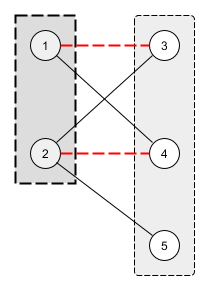
\includegraphics[width = 0.2\textwidth] {img/TobiasT_Laufzeit.jpg}
	\end{figure}
\end{frame}

\begin{frame}{Modelierung}
	\begin{itemize}
		\item Beispiel: Guardian of Decency (Competitive Programming 3, Seite 182)
		\item (Je nach verbleibender Zeit:) noch mehr Graphentheorie: bipartit $< == >$ keine ungeraden Kreise, ...
	\end{itemize}
\end{frame}

\end{document}
